\documentclass[12pt]{article}

\usepackage[letterpaper,margin=0.75in]{geometry}

\usepackage[outputdir=../dist]{minted}

\usepackage{amsmath}
\usepackage{booktabs}
\usepackage{graphicx}
\usepackage{listings}
\usepackage{fancyhdr}
\usepackage{standalone}
\usepackage{float}
\usepackage{hyperref}
\usepackage[style=vancouver]{biblatex} %Imports biblatex package

% Bibliography
\addbibresource{all.bib}

\setlength{\parindent}{0pt}

\pagestyle{fancy}

\begin{document}

\lstset{
  language=Python,
  basicstyle=\small,          % print whole listing small
  keywordstyle=\bfseries,
  identifierstyle=,           % nothing happens
  commentstyle=,              % white comments
  stringstyle=\ttfamily,      % typewriter type for strings
  showstringspaces=false,     % no special string spaces
  numbers=left,
  numberstyle=\tiny,
  numbersep=5pt,
  frame=tb,
}

\title{PX2505 - Optics Lab Report - Newton Rings }
\date{}
\def\theinstructor{}



\author{Sidney Pauly}
\def\theuoastudentid{52104132}

\makeatletter

\let\thetitle\@title
\let\theauthor\@author
\let\thedate\@date


\makeatother




\fancyhf{}
\fancyhead[L]{\today}
\fancyhead[C]{Name: \theauthor}
\fancyhead[R]{ID: \theuoastudentid}

\fancyfoot[C]{\thepage}
% \maketitle

\begin{titlepage}
  \begin{center}
    \Large
    \textbf{\thetitle}
        
    \vspace{0.4cm}
    \large
    \thetitle
        
    \vspace{0.4cm}
    \textbf{\theauthor}\\
    \textbf{\theuoastudentid}\\
    \textbf{\today}\\

       
    \vspace{0.9cm}

  \end{center}

  \vfill

  \begin{center}

    University of Aberdeen\\
    Scotland\\
    UK\\
    \thedate
    \vspace{0.4cm}
    \url{https://github.com/sidney-pauly/papers}
  \end{center}
\end{titlepage}

\tableofcontents

\section{Aims}

The aim of this experiment was to examine light interference at thin-film interfaces.
This sort of interference can
happen between curved surface (like a lens) on top of a flat surface with a small gap between them.
Due to the produced rings (caused by the interference minima and maxima) this phenomena
is called "Newton Rings".\\
\\
Beyond studying the phenomena itself further aims of the experiment are:
\begin{enumerate}
  \item Comparing the accuracy of different measurement procedures (manual vs. image based)
  \item Analyzing the geometry of the produced pattern to measure the curvature of the used lens
  \item Measuring the refractive index of a different material (water). This can be done by placing it into the gap and
        using the obtained curvature measurement to calculate the refractive index.
\end{enumerate}

\section{Theory}

\subsection{Interference}

The newton rings experiment is an experiment on interference. What is special about
the interference that can be observed is that it does not require a coherent light
source (like a laser). Instead it creates the interference by splitting the light
(partly reflecting it and partly letting it through) and thereby letting it travel
different distances (within the range of one wavelength).\\

\begin{figure}[H]
  \centering
  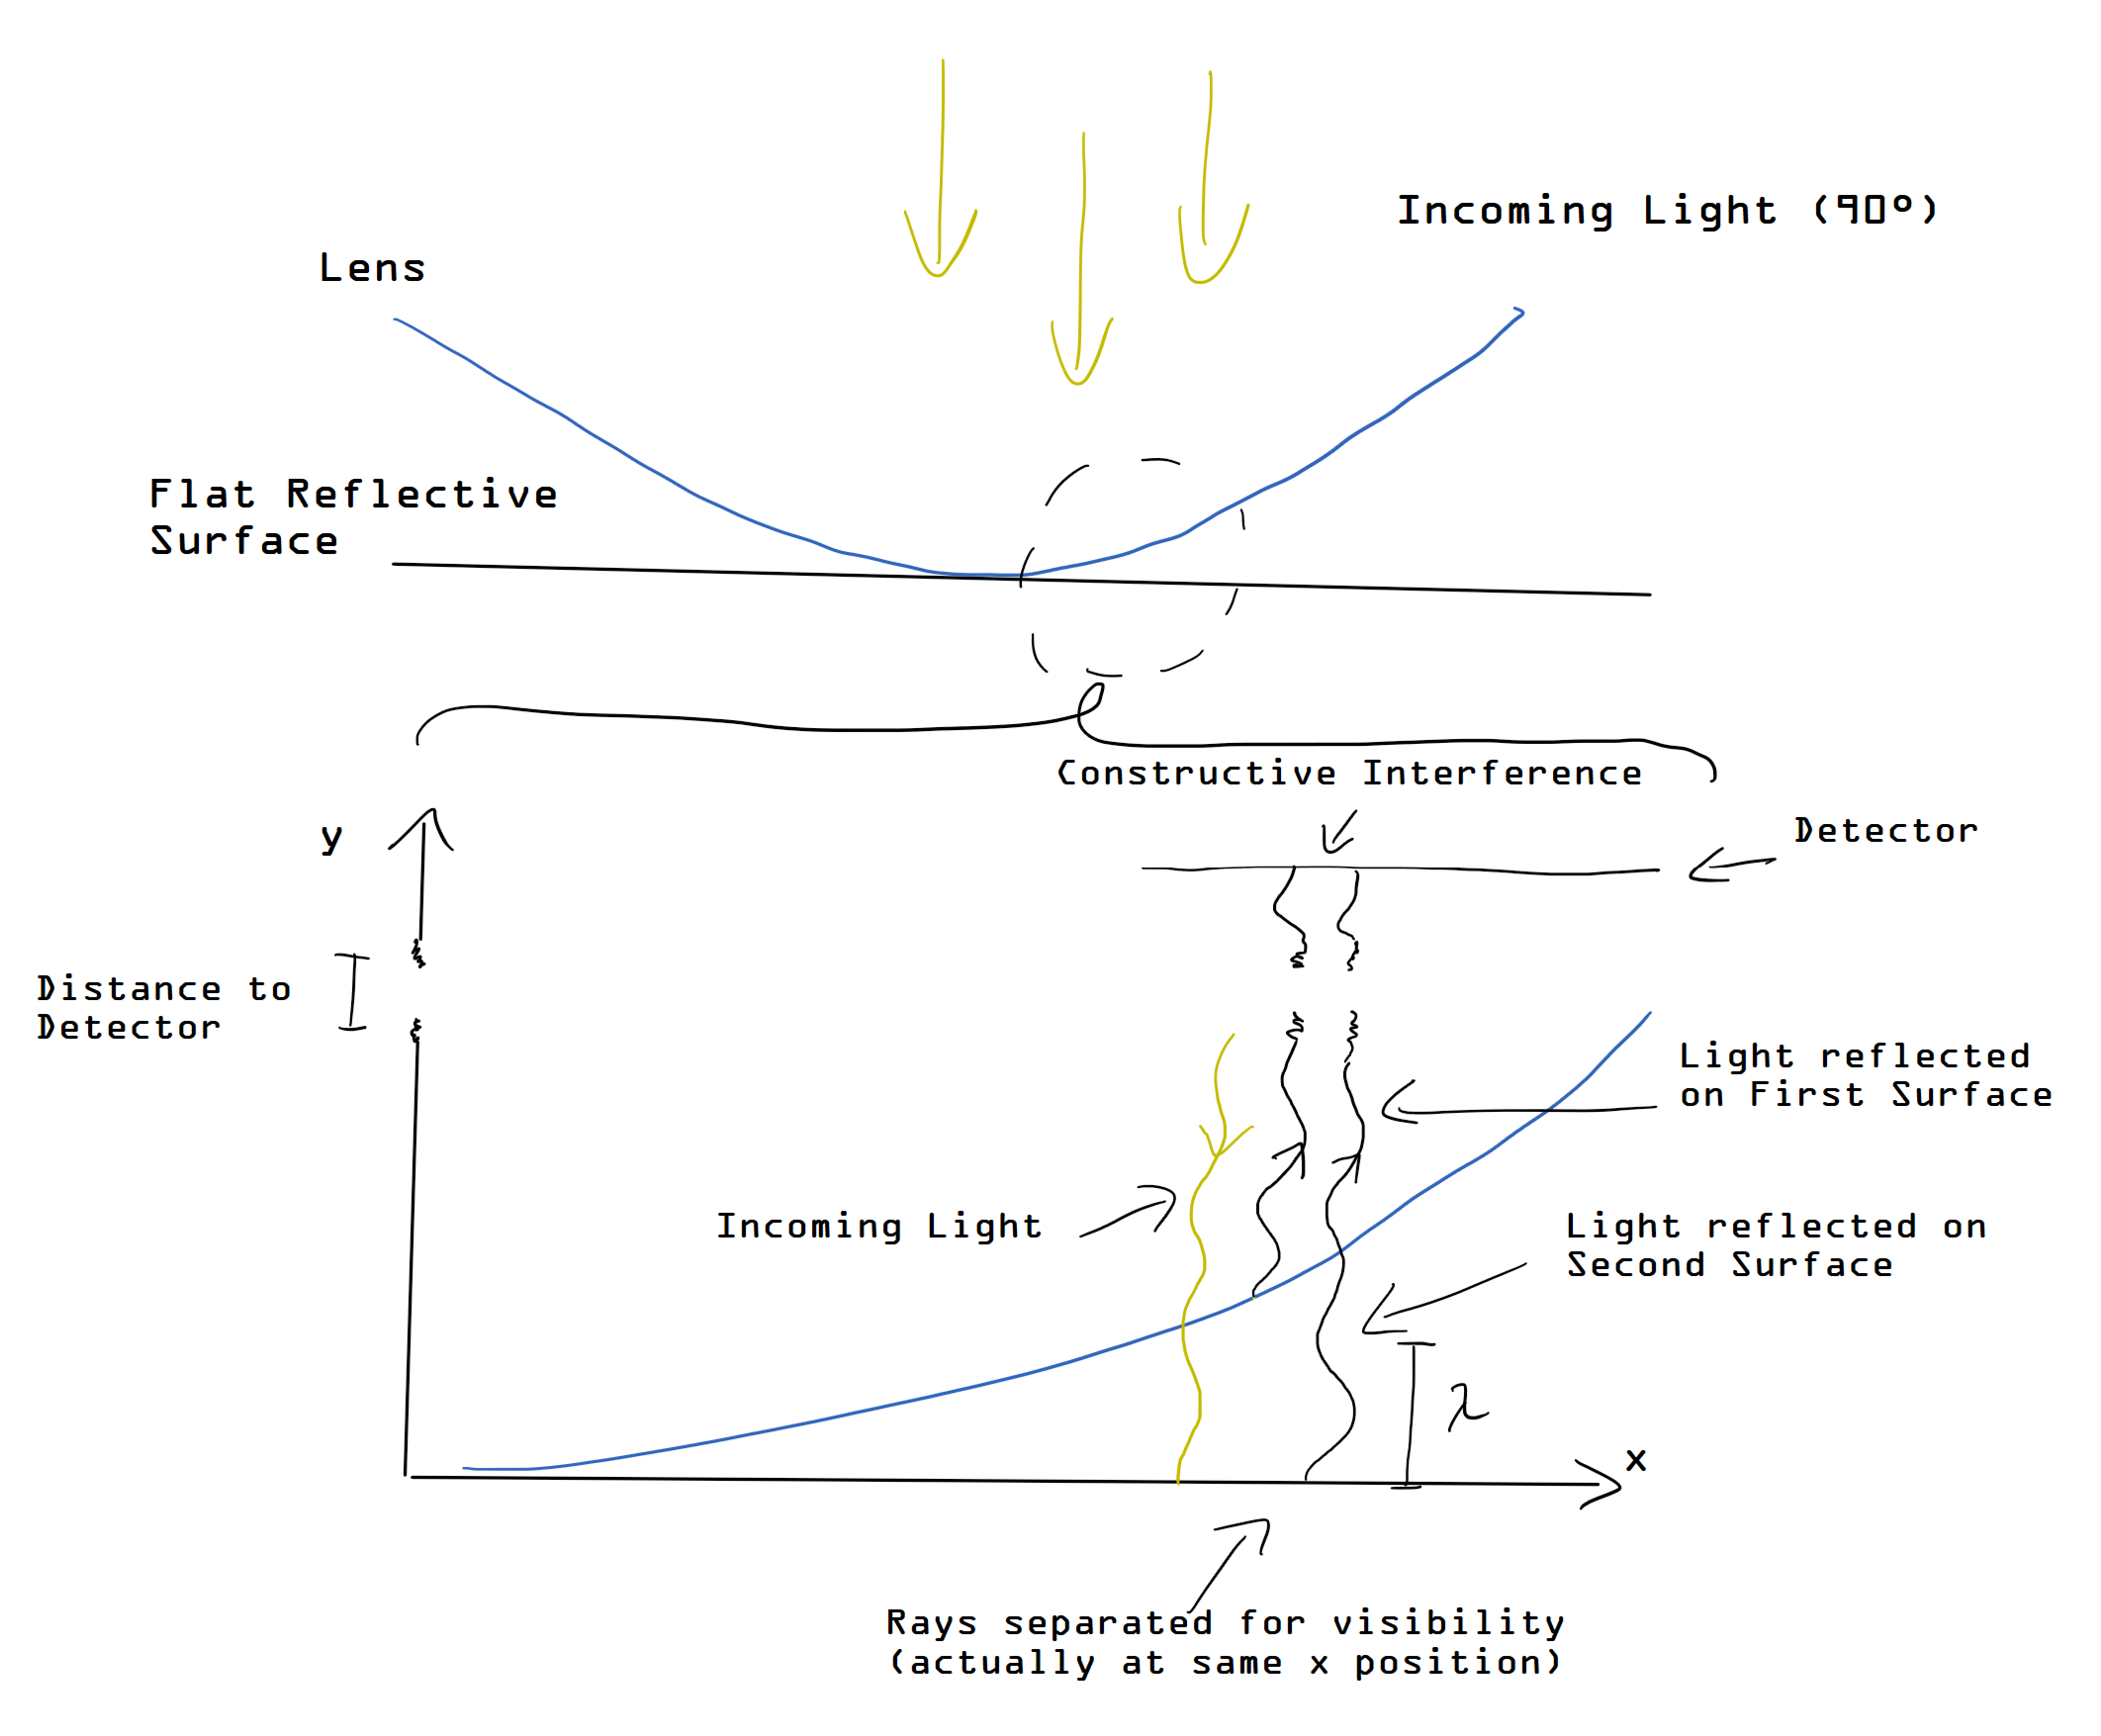
\includegraphics[width=17cm]{./images/theory.png}
  \caption{Light path through the Lens and Reflective surface resulting in interference}
  \label{fig:theory}
\end{figure}

To get a single light beam to travel different distances, a semi reflecting surface
is used. Some light travels through the reflective surface and while other light gets
transmitted the transmitted light is then reflected back at a further reflecting surface
within a few wavelength in distance. If the reflective surface is exactly an integer
multiple of ½ the wavelength away, the light will interfere constructively (as it has
to go back and forth thereby covering an integer multiple of the wavelength).
Conversely for values of ¼ integer multiple of the wavelength the light will interfere
destructively as it now is shifted half a wavelength. This works with non-coherent light, as each 
packet of light is interfering with itself, rather than with other light beams. This
also means that this interference can only happen, if the distance between the half 
reflecting surface and the reflective surface is small enough, as otherwise the light 
with the longer path length will take too long as each packet of light is limited in length.\\
\\
It should also be noted that different materials between the surfaces will alter the effective 
path length the light has to take and will thus alter at what distances destructive and 
constructive interference happens. This fact will later be used to measure the refractive index of water.\\
\\
In the actual experiment a lens is used, as the semi reflective surface. 
This has the advantage of directing the light only exactly downwards, 
preventing any transverse components to affect the result. Additionally using a
lens means that the distance between semi reflective surface and substrate starts from 0 and 
progressively gets bigger away from the contact point. Therefore at different distances form 
the center there is different amounts of interference. If the light is monochromatic this
will create a clear interference pattern, which can be measured and used to infer the refractive
index in the gap (if the refractive index is known other properties could of course also be inferred)\\
\\
Furthermore it is important that the lens reflects and transmits close to  50\% of the light. 
This is because the visibility of any interference pattern is best if the relative intensity
of the two beams involved is equal \autocite{ross}.\\
\\

\subsection{Geometry}

As previously mentioned the it is possible to derive the curvature of the lens from the
produced interference pattern. The Lab Manual\autocite{ross} provides the following formula:

\begin{equation}
  R = \frac{r^2}{m}\frac{n}{\lambda}
  \label{eq:lens_curvature}
\end{equation}

Here $R$ stands for the radius of the lens. $\lambda$ is the wavelength of the light and $n$ the 
refractive index of the material between the lens and the substrate.
$\frac{r^2}{n}$ as the ratio between the number of the maxima
($n$) and the radius of that maxima ($r$). The maximas are rings in the interference patterns with the
fewest light. Figure \ref*{fig:sodium_pattern} shows an interference pattern. The maximas appear as bright
rings around the center. 


\begin{figure}[H]
  \centering
  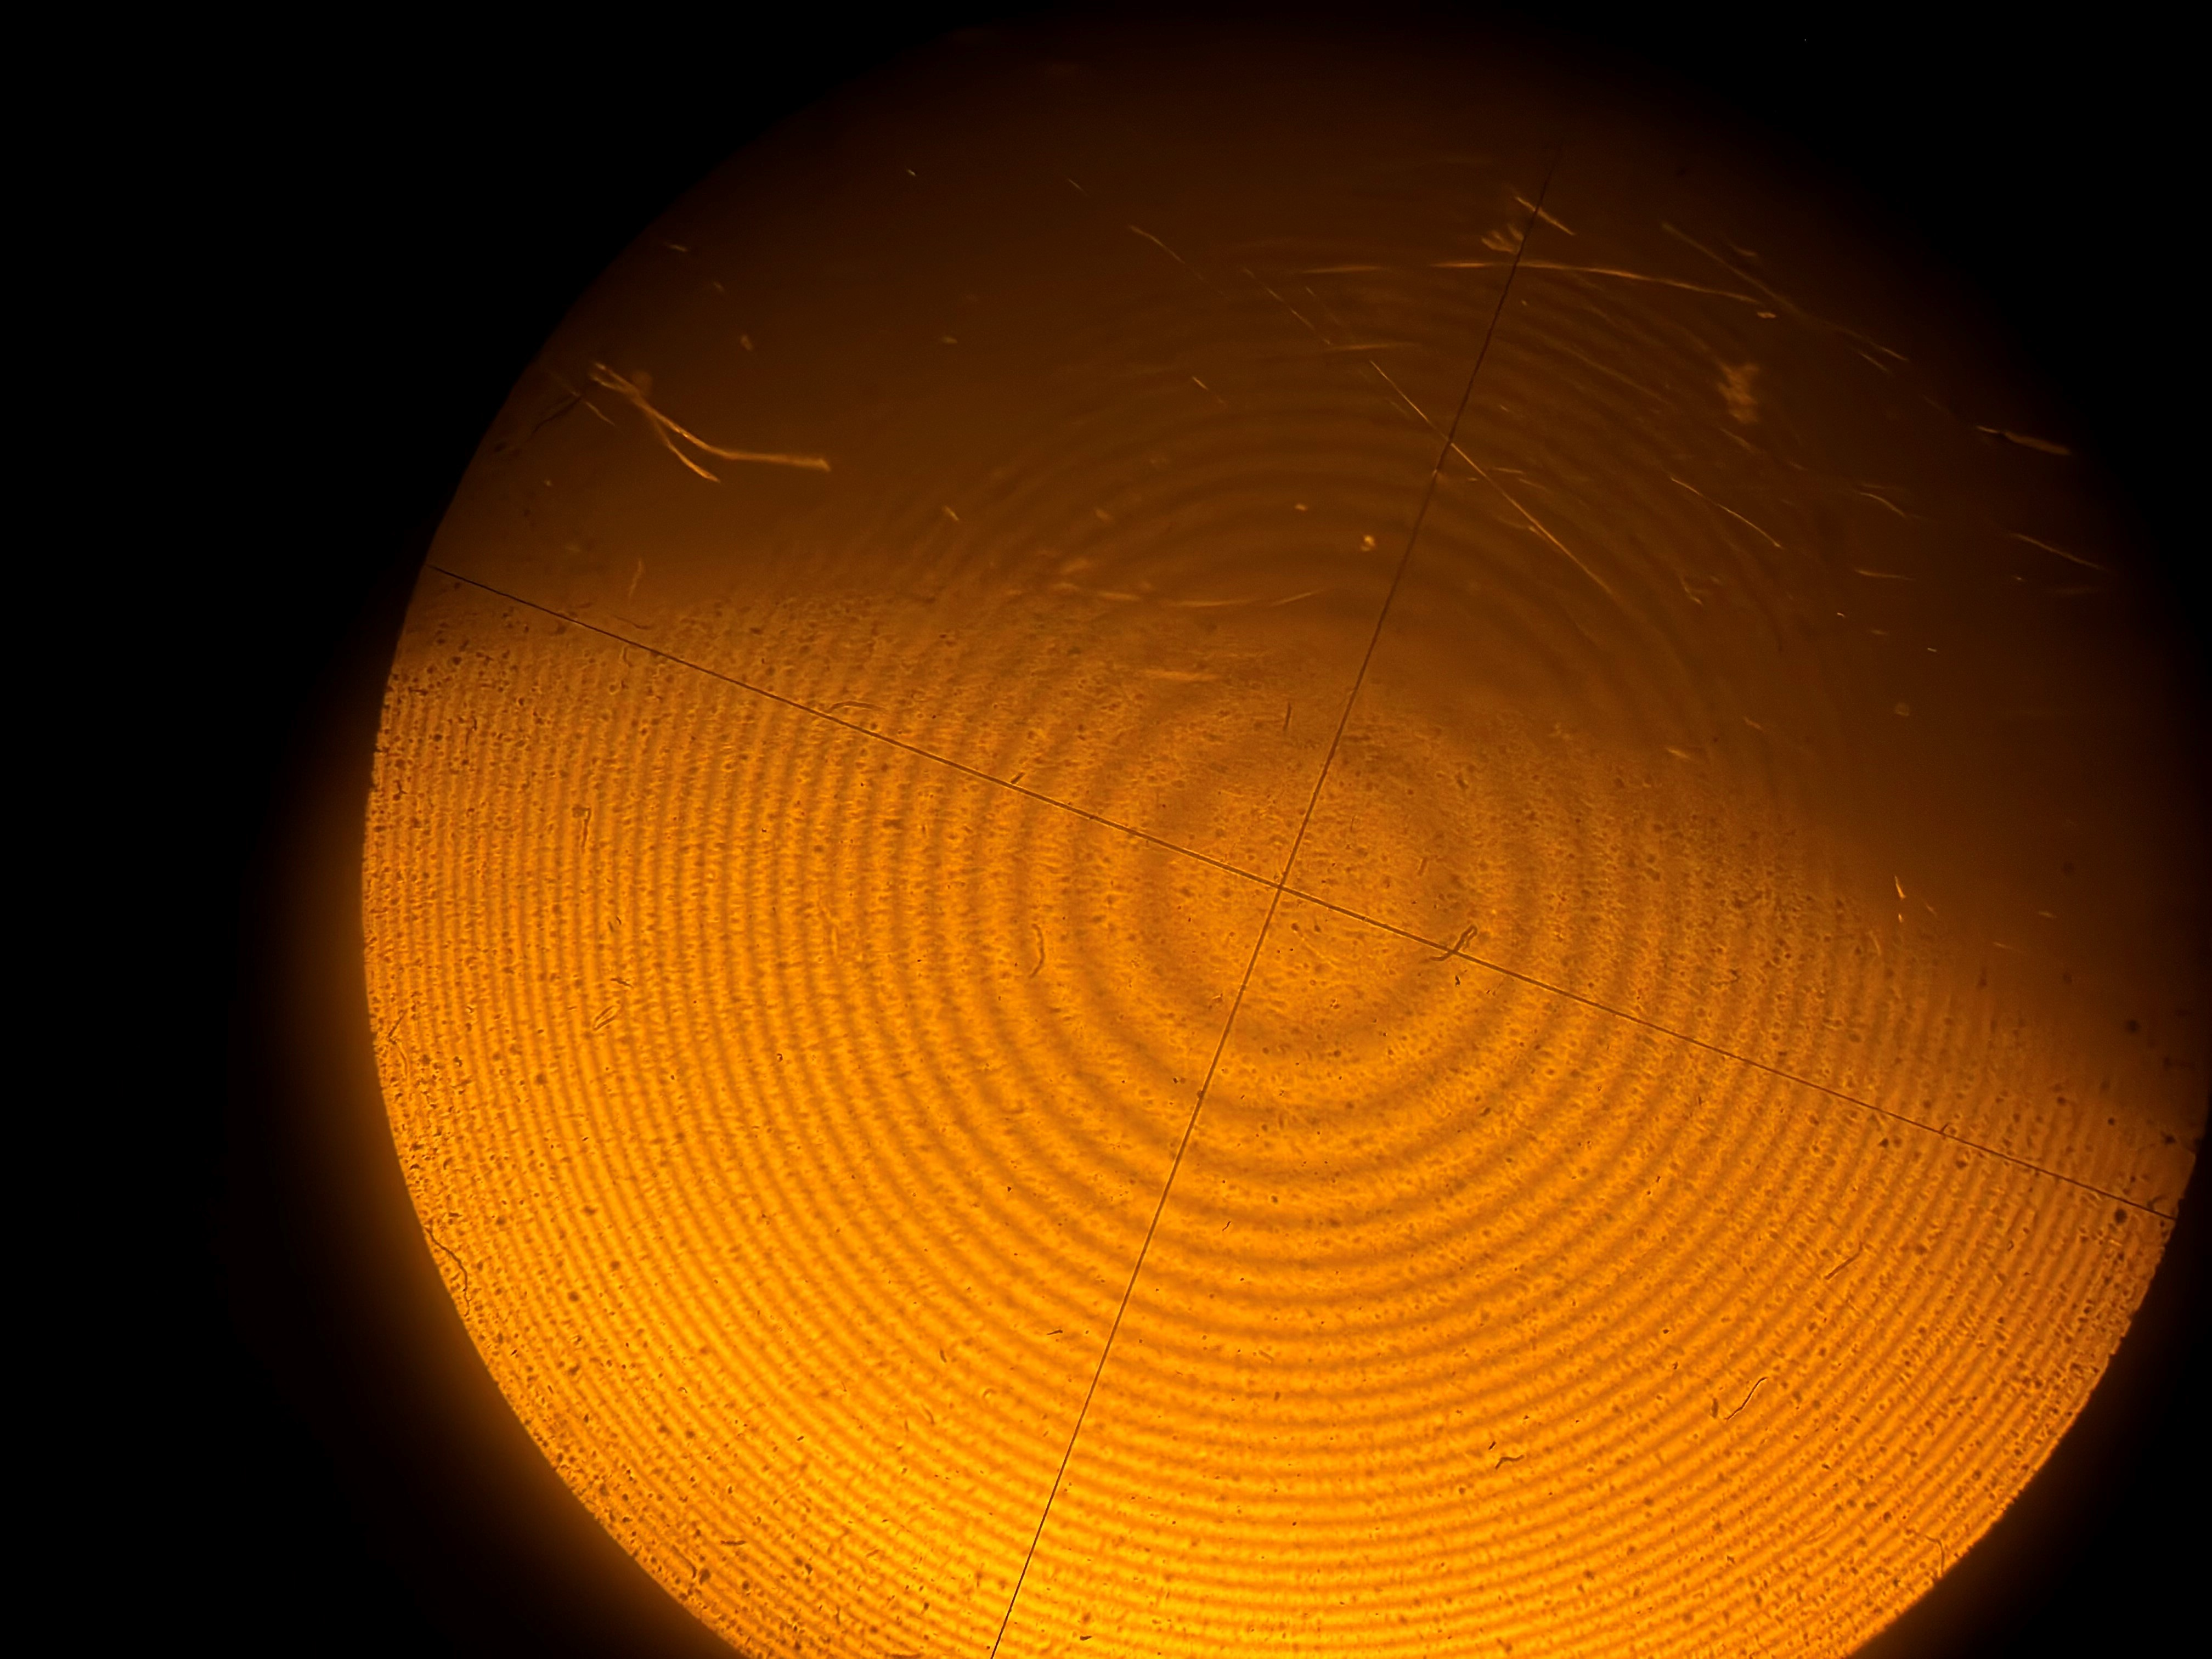
\includegraphics[width=12cm]{./images/sodium_pattern.jpeg}
  \caption{Fringes produced in the experiment}
  \label{fig:sodium_pattern}
\end{figure}


In a first step the experiment is run with air in the gap. As air has a known refractive index
of $n = 1$. Furthermore a monochromatic sodium light source is used, which has a known wavelength
of $\lambda = 589.3 nm$\autocite{ross} the curvature can be calculated. Now if a different material is to be examined it is
possible to solve the formula based on the known curvature:
\begin{equation}
  n = R \lambda \frac{m}{r^2}
  \label{eq:refractive_index}
\end{equation}

\section{Method}

\subsection{Overall setup}

\begin{figure}[H]
  \centering
  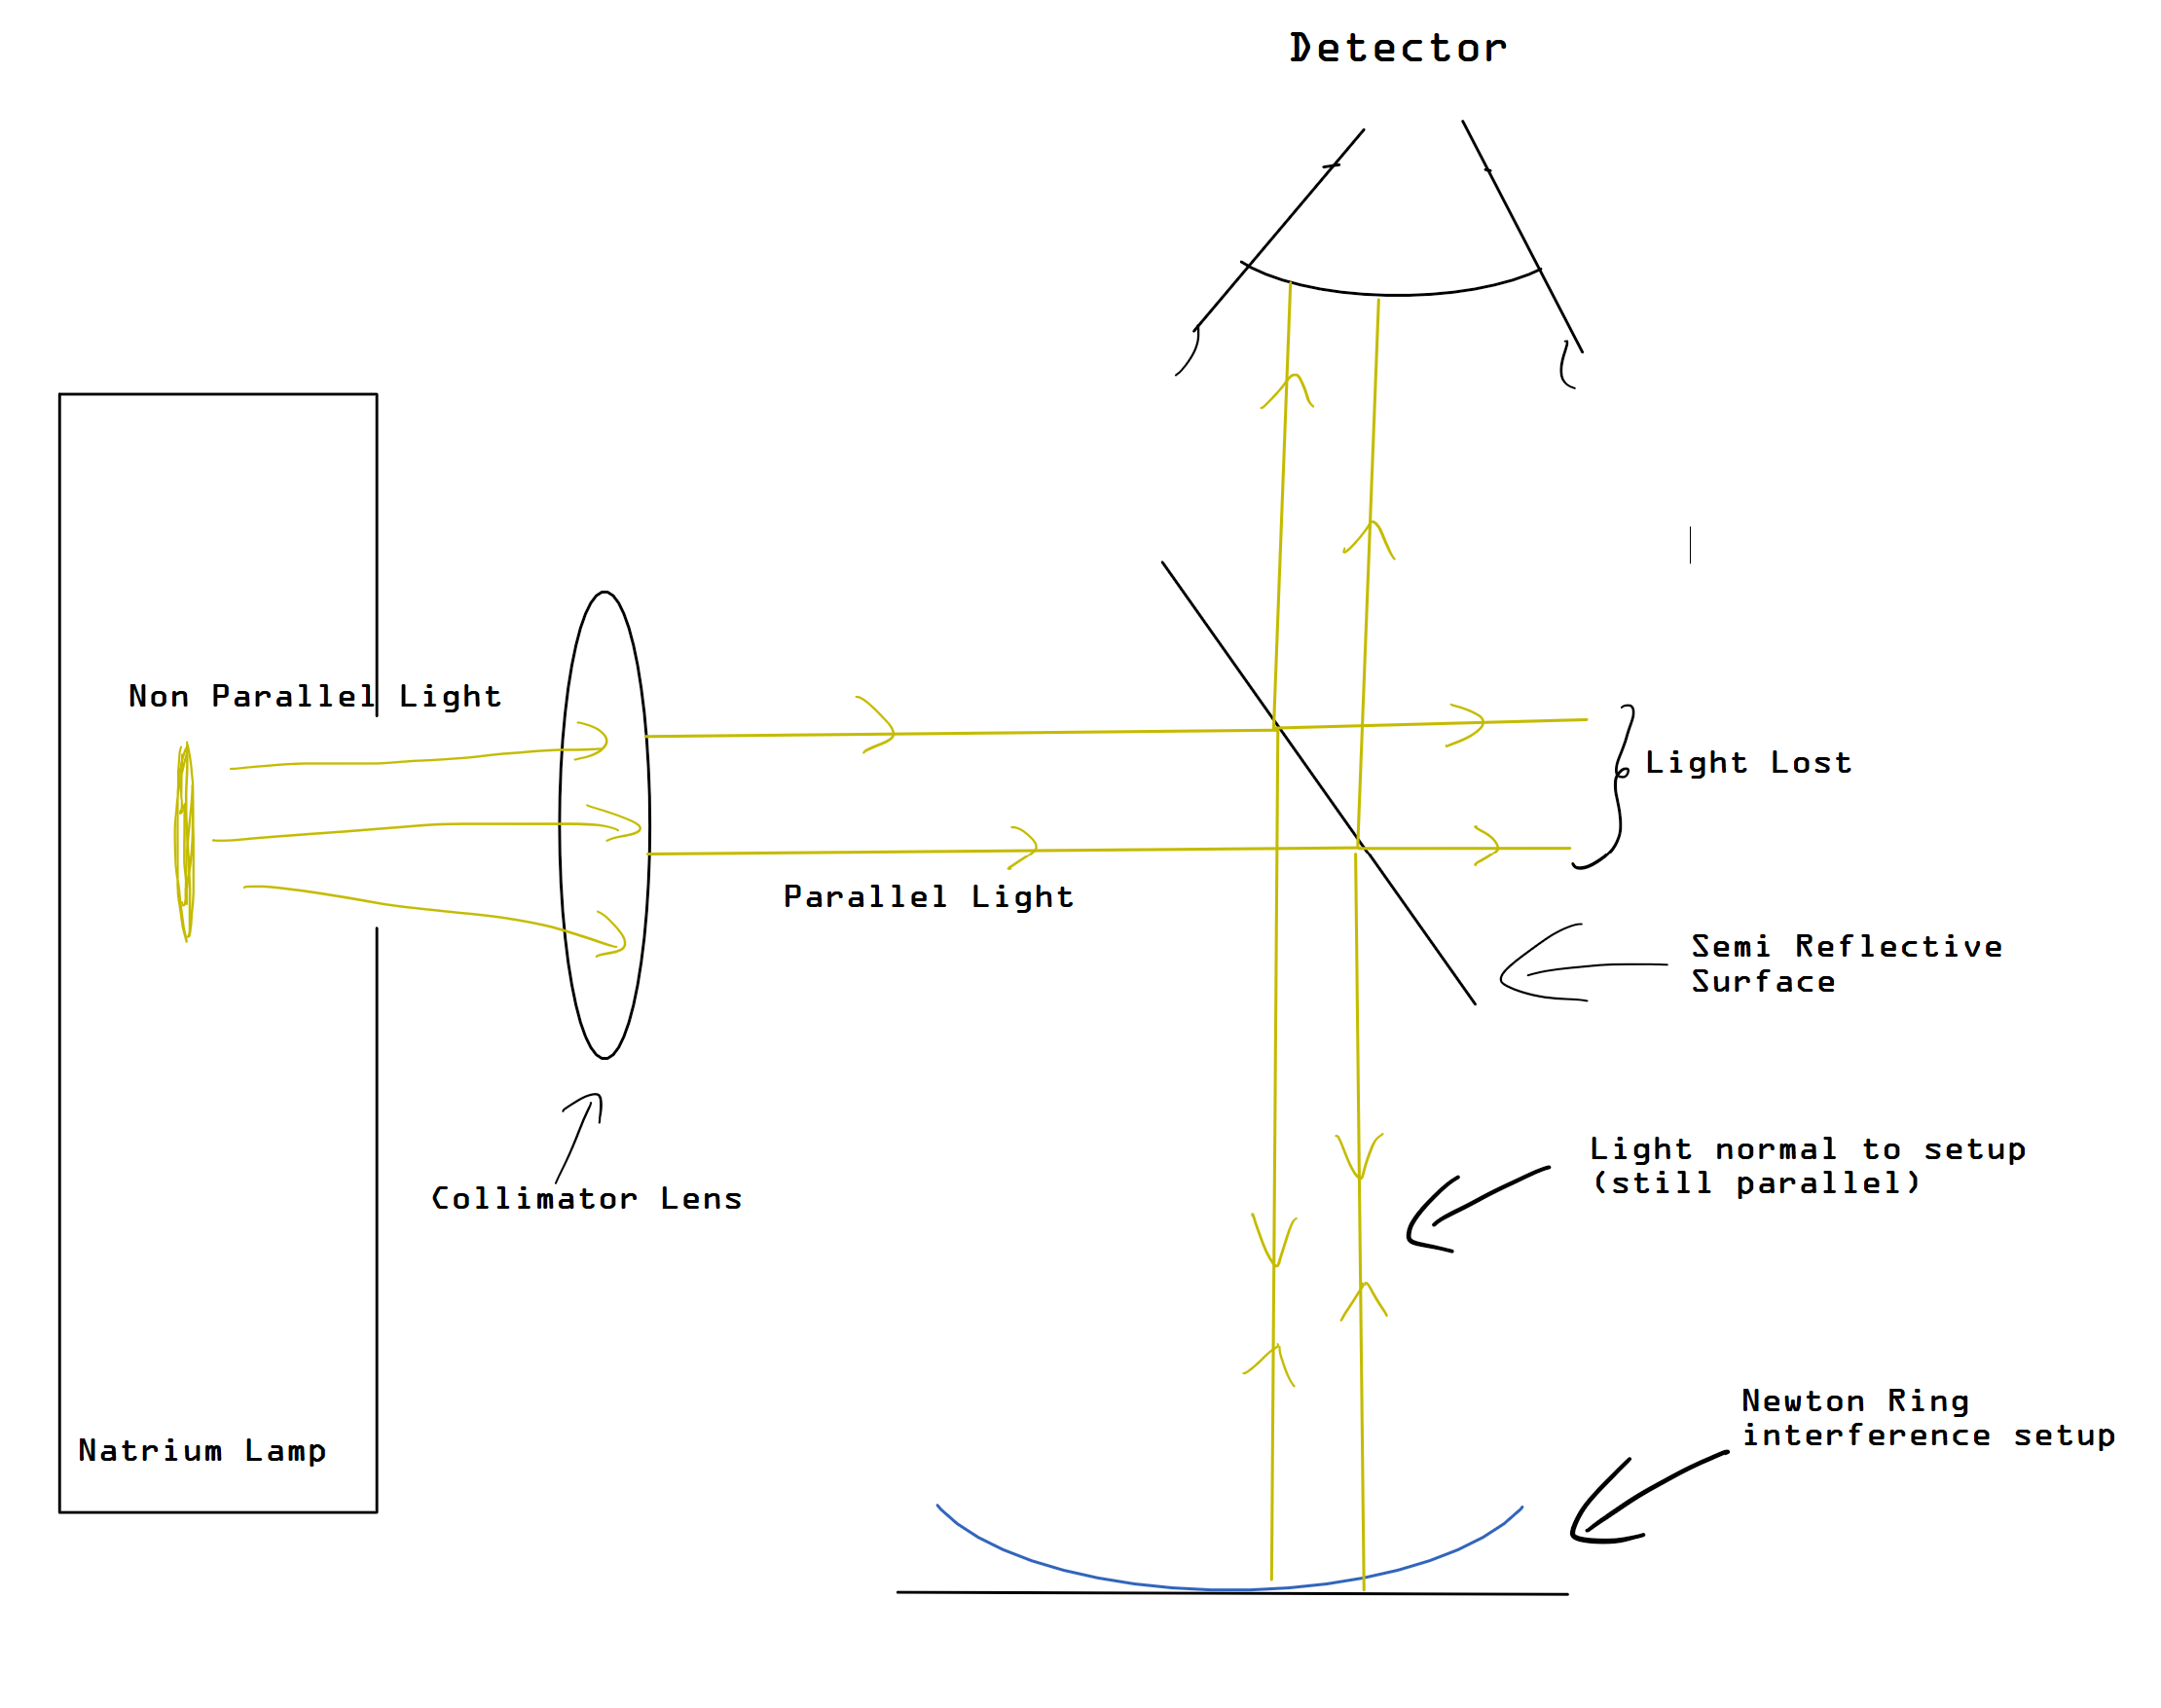
\includegraphics[width=17cm]{./images/setup.png}
  \caption{The experimental setup}
  \label{fig:setup}
\end{figure}

As described for such interference to happen it is not necessary to have coherent light.
Therefore in the experiment a “normal” sodium lamp can be used. On the other hand it is
important that the light comes from exactly above and that all light rays are parallel to
ensure that the resulting interference can be clearly related back to the geometry of the
lens. In other words it is important to ensure that light that did not experience the
same amount of interference does not end on top of each other on the detector. To
ensure that the light is parallel a collimator lens is used. Getting the light to shine 
onto the lens at 90 degrees is a bit more complicated, as that would usually result
in the resulting interference pattern to be reflected directly back into the light source.
To sperate light source and detection spot an additional semi-reflecting surface is
used at 45 degrees. It first reflects the light from the lamp downwards onto the lens. 
The resulting interfering light then travels back upwards and is partially transmitted 
through to the detector (some of it, is still reflected into the source, but this just reduces
the overall brightness).

\subsection{Manual measurements}

\begin{figure}[H]
  \centering
  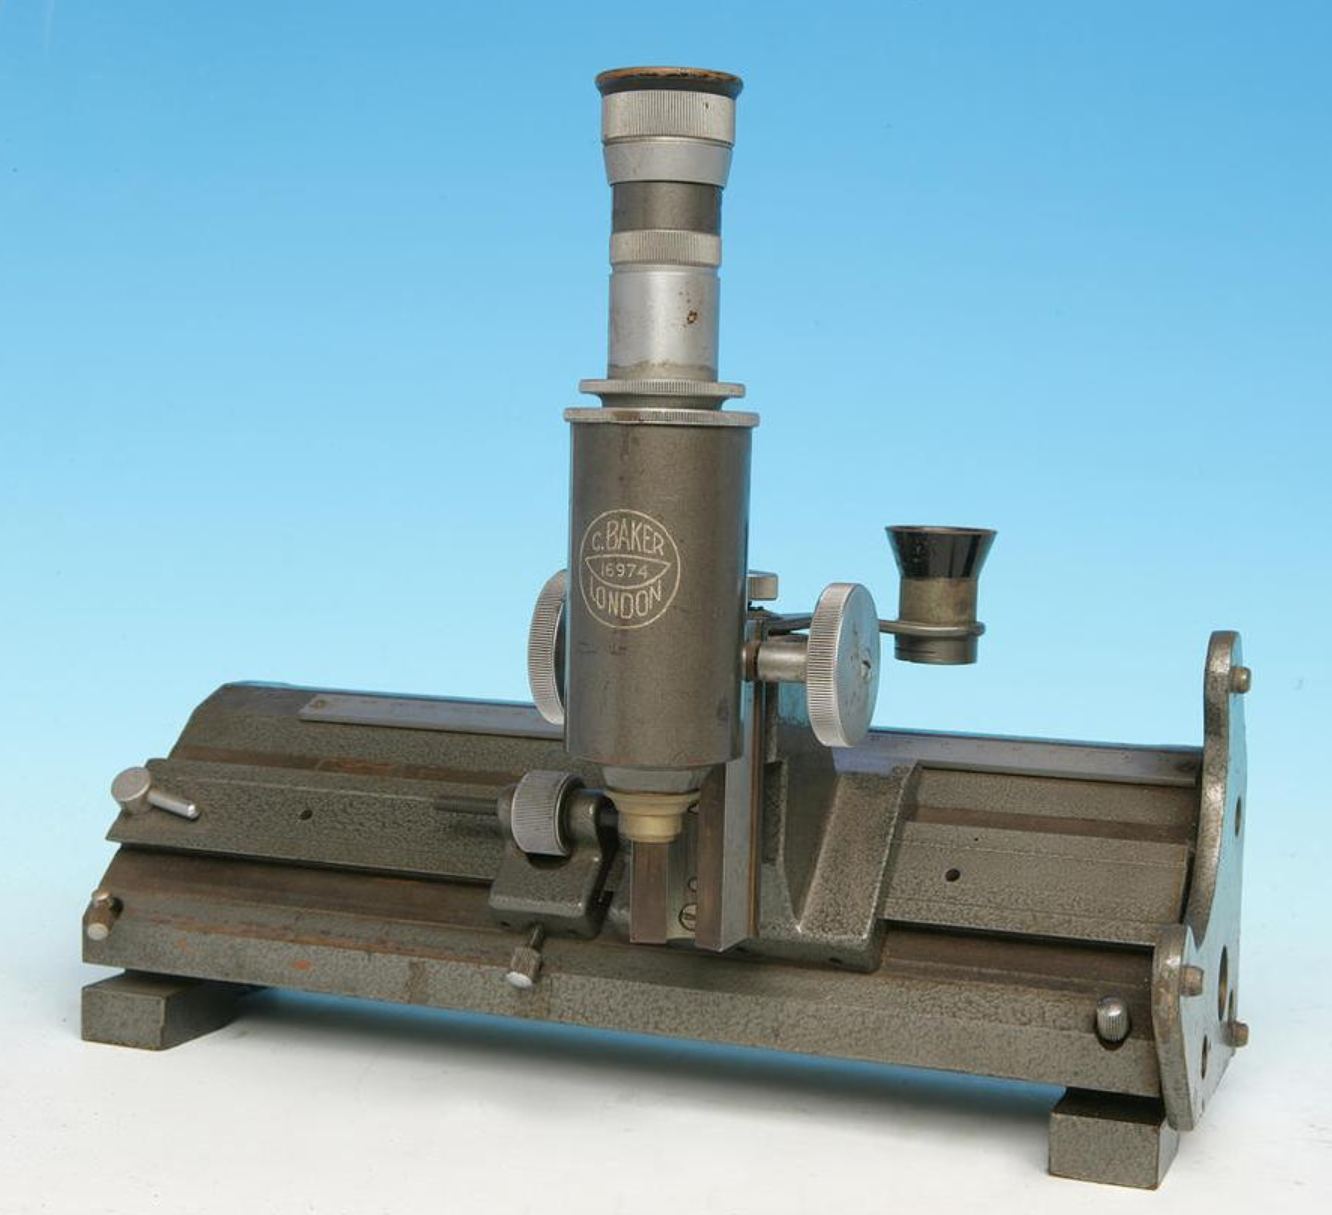
\includegraphics[width=12cm]{./images/traveling_microscope.png}
  \caption{A traveling microscope\autocite{leeds}}
  \label{fig:traveling_microscope}
\end{figure}


The first method to determine the radius of the produced maxima rings is manual measurement.
It can be done through the use of a traveling microscope (See Figure \ref{fig:traveling_microscope}).
A traveling microscope can be finely
adjusted along its axis. These microscopes also include a vernier scale, thus the current
position can be read to a hight accuracy. \\
\\
To position the microscope exactly over an image feature the microscope has a build in crosshair. 
It can be seen in Figure \ref*{fig:sodium_pattern}.

\subsection{Image based measurements}

The second method to get the measurements is to take a picture of the interference pattern. The size of
different features in the picture can then be related to their physical size.\\
\\
Taking these measurements is made easier through the utilization fo digital software like ImageJ\autocite{ImageJ}
The software allows to load a digital image and then measure length within the image. In order to
relate these distances to physical distance a known length within the image needs to be provided first.
This can be done by taking a picture of a ruler at the exact same spot as the lens\footnote{A helping characteristic
of microscopes is that only objects at a narrow distance interval are in focus. Thus if the ruler is in focus it is 
very close to the height that the lens was at.}:

\begin{figure}[H]
  \centering
  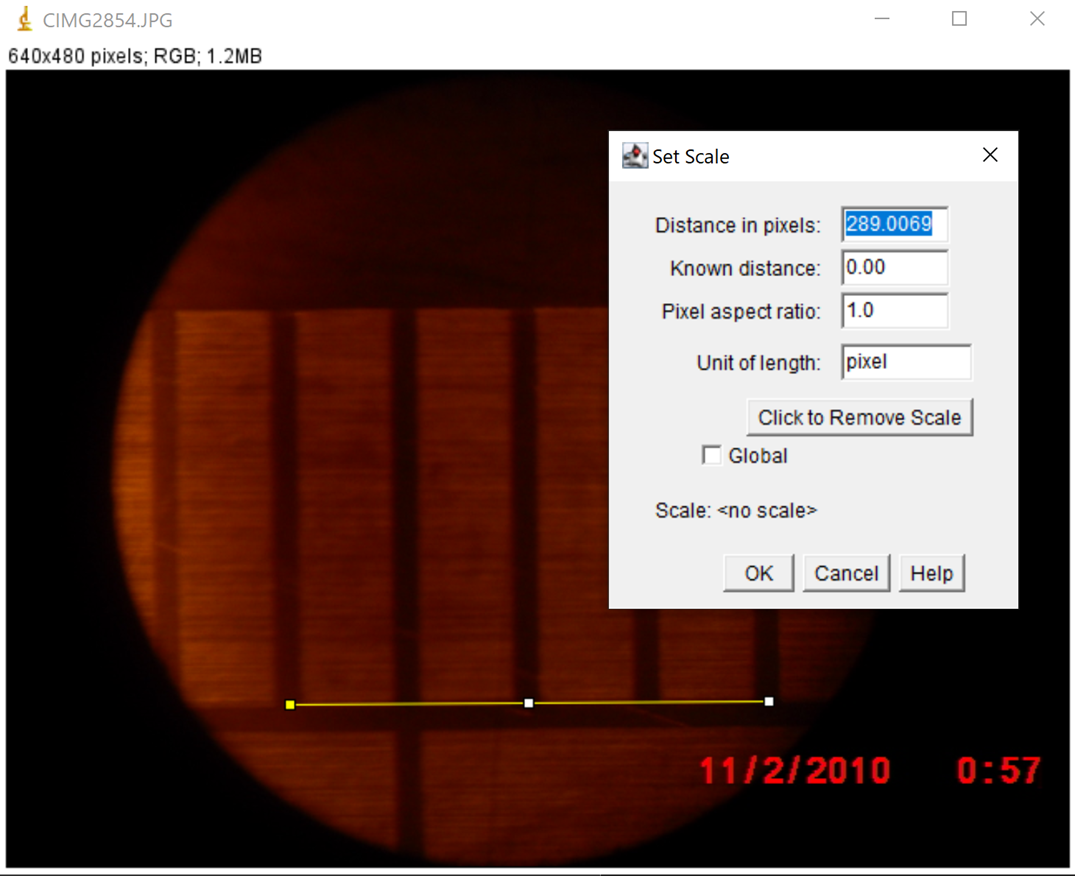
\includegraphics[width=10cm]{./images/imagej_measure_ruler.png}
  \caption{Providing a known physical distance within ImageJ}
  \label{fig:imagej_provide_ditance}
\end{figure}

As shown in Figure \ref{fig:imagej_provide_ditance} a distance on the ruler can then be measured and
the known distance value (here 4mm) can be provided to the software.\\
\\
Now the image to be analyzed can be loaded into the software. One way of then measuring the size
of features would be to find them on the screen and use the distance tool. However it is faster
and more precise to use the "Plot profile" feature. It produces a graph of the brightness of each
pixel along a drawn line:

\begin{figure}[H]
  \centering
  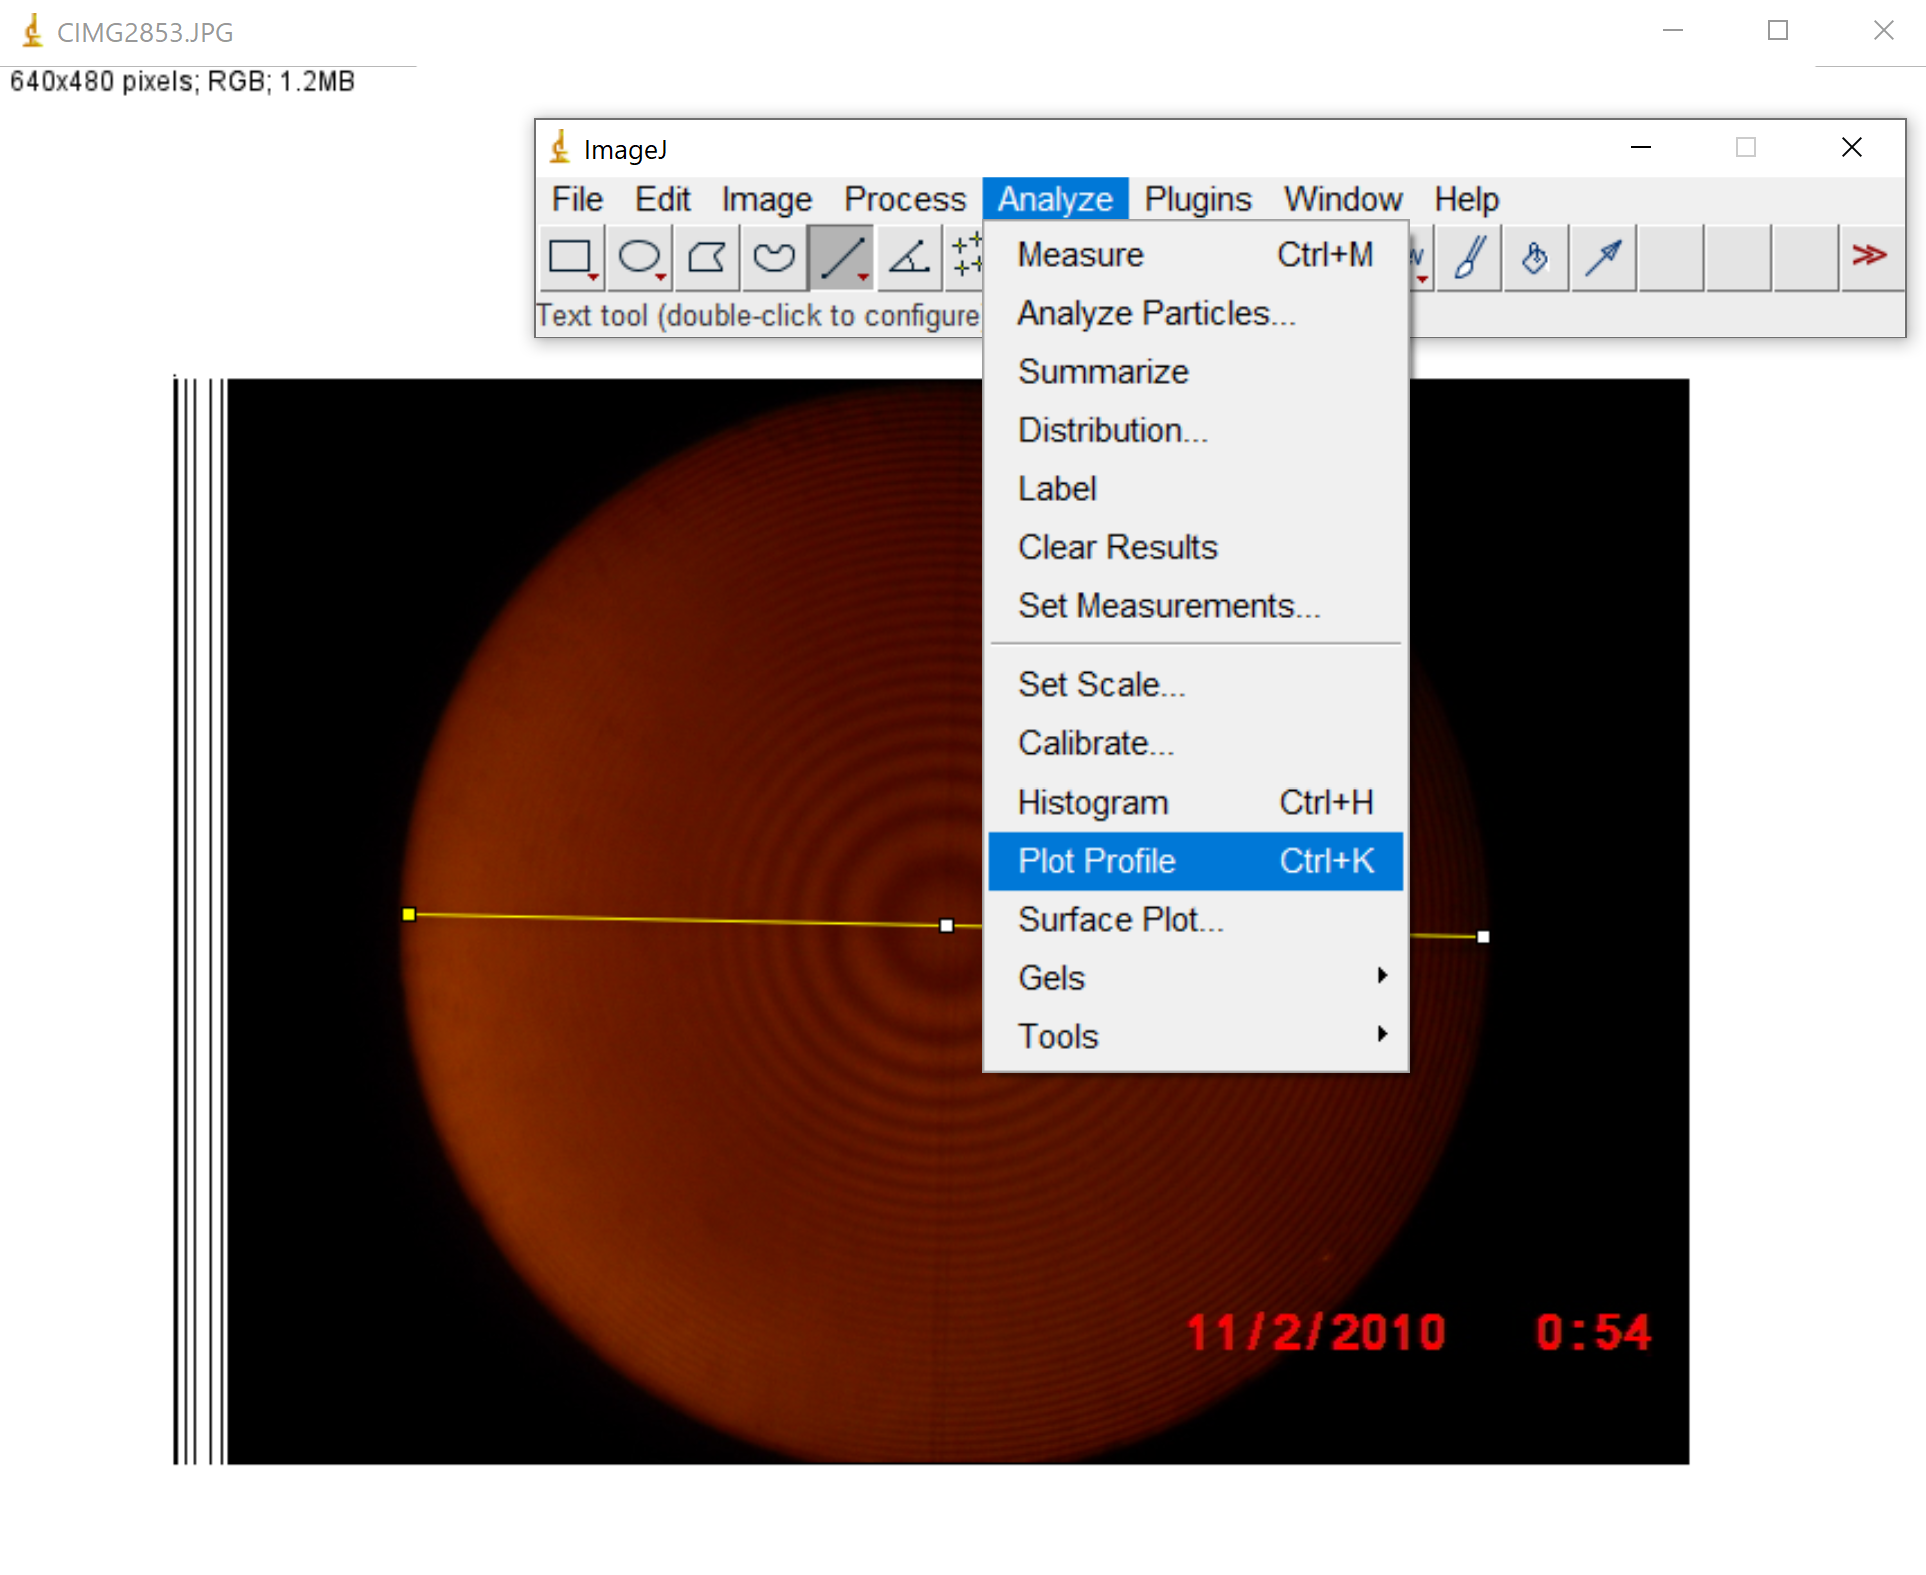
\includegraphics[width=10cm]{./images/imagej_plot_profile.png}
  \caption{ImageJ's "Plot Profile" feature}
  \label{fig:imagej_plot_profile}
\end{figure}

\section{Results}

\subsection{White light}

In addition to examining the fringes produced by a sodium lamp the setup
was tested with a white light source. The resulting fringes looked like this:

\begin{figure}[H]
  \centering
  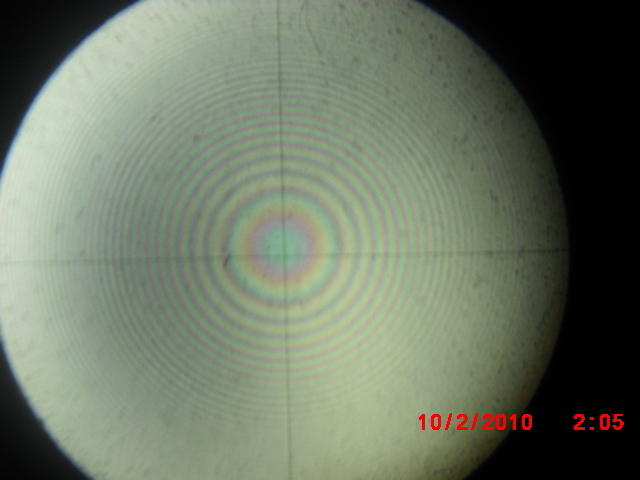
\includegraphics[width=12cm]{./images/white_light.JPG}
  \caption{Interference pattern produced by a white light source}
  \label{fig:white_light}
\end{figure}

\subsection{Manual measurements}
Through measuring the distances between different maxima of the interference pattern
it is possible to determine the refractive index of the material in between the gap
or the curvature of the lens used (depending on which of the two is unknown).
The following measurements where taken by moving the traveling microscope over the different features:

\begin{table}[H]
  \begin{tabular}{lllll}
  Ring Number & Left Hand Side (mm) & Right Hand Side (mm) & Diameter 2y (mm) & $y^2$ ($mm^2$) \\
  \hline
  2           & 92.46               & 91.42                & 1.04             & 0.2704                                       \\
  4           & 92.94               & 90.92                & 2.02             & 1.0201                                       \\
  6           & 93.24               & 90.62                & 2.62             & 1.7161                                       \\
  8           & 93.48               & 90.38                & 3.1              & 2.4025                                       \\
  10          & 93.72               & 90.16                & 3.56             & 3.1684                                       \\
  12          & 93.9                & 89.96                & 3.94             & 3.8809                                       \\
  14          & 94                  & 89.8                 & 4.2              & 4.41                                         \\
  16          & 94.22               & 89.62                & 4.6              & 5.29                                         \\
  18          & 94.4                & 89.48                & 4.92             & 6.0516                                       \\
  20          & 94.54               & 89.3                 & 5.24             & 6.8644                                      
  \end{tabular}
\end{table}

The ring number denotes the interference maxima that was measured. “Left Hand Side” is
the traveling microscope reading on the left side of the ring, “Right Hand Side”
the reading of the right side of the maxima. Through this the diameter of the maxima
can be determined and thereby its radius r, which is basically its distance from the
contact point of lens and reflecting substrate.

Through the use of excel the following fit can then be done find $\frac{r^2}{m}$:

\begin{figure}[H]
  \centering
  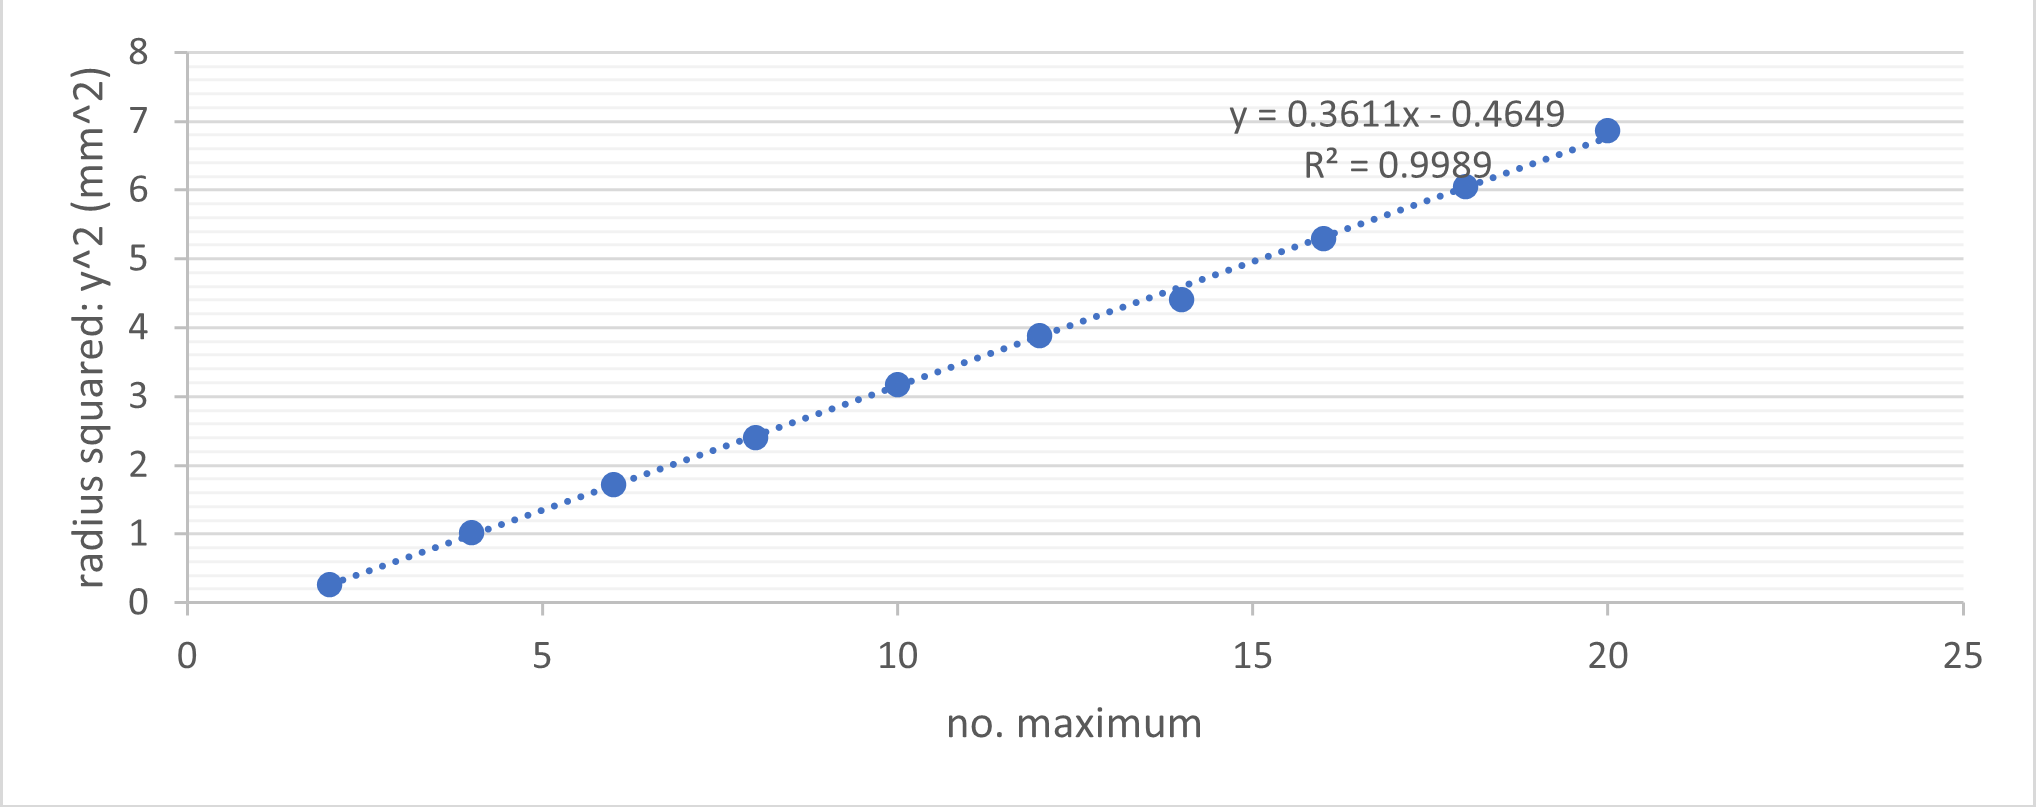
\includegraphics[width=16cm]{./images/results_manual.png}
  \caption{$m$ vs. $r^2$ and slope fit obtained through manual measurements}
  \label{fig:result_manual}
\end{figure}

The values of the resulting trend line can be seen directly on the graph. An $R^2$  value of 0.9989
is high and is indicative precise measurements (For statistically perfect data  the value would be 1).\\

The gradient of the slope ($\frac{r^2}{m} = 0.3611mm^2$) can then be plugged into Formula \ref{eq:lens_curvature} to
obtain a radius of the lens $R$ of $61.3cm$.

\subsection{Image analysis}

As described this analysis can also be done by utilizing the ImageJ software. The previously
mentioned "Plot Profile" tool provided us with a brightness graph that looked like this:

\begin{figure}[H]
  \centering
  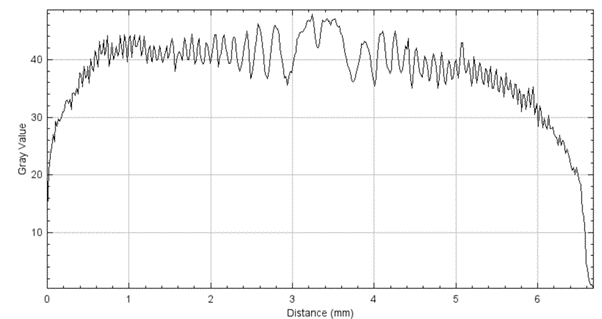
\includegraphics[width=14cm]{./images/profile.png}
  \caption{Brightness values across the interference pattern}
  \label{fig:profile}
\end{figure}

Measuring the distances between the different peaks the following values where obtained:

\begin{table}[H]
  \begin{tabular}{lllll}
  \hline
  Ring Number & Left Hand Side (mm) & Right Hand Side (mm) & Diameter 2y (mm) & $y^2$ ($mm^2$) \\
  \hline
  2           & 2.8200              & 3.5110               & 0.6910           & 0.11937025                                   \\
  4           & 2.253               & 4.092                & 1.8390           & 0.84548025                                   \\
  6           & 1.908               & 4.424                & 2.5160           & 1.582564                                     \\
  8           & 1.645               & 4.673                & 3.0280           & 2.292196                                     \\
  10          & 1.424               & 4.908                & 3.4840           & 3.034564                                     \\
  12          & 1.244               & 5.101                & 3.8570           & 3.71911225                                   \\
  14          & 1.051               & 5.267                & 4.2160           & 4.443664                                     \\
  16          & 0.885               & 5.433                & 4.5480           & 5.171076                                     \\
  18          & 0.719               & 5.585                & 4.8660           & 5.919489                                     \\
  20          & 0.581               & 5.783                & 5.2020           & 6.765201                                     \\
  \end{tabular}
\end{table}

Plotting these values leads to the following best fit:

\begin{figure}[H]
  \centering
  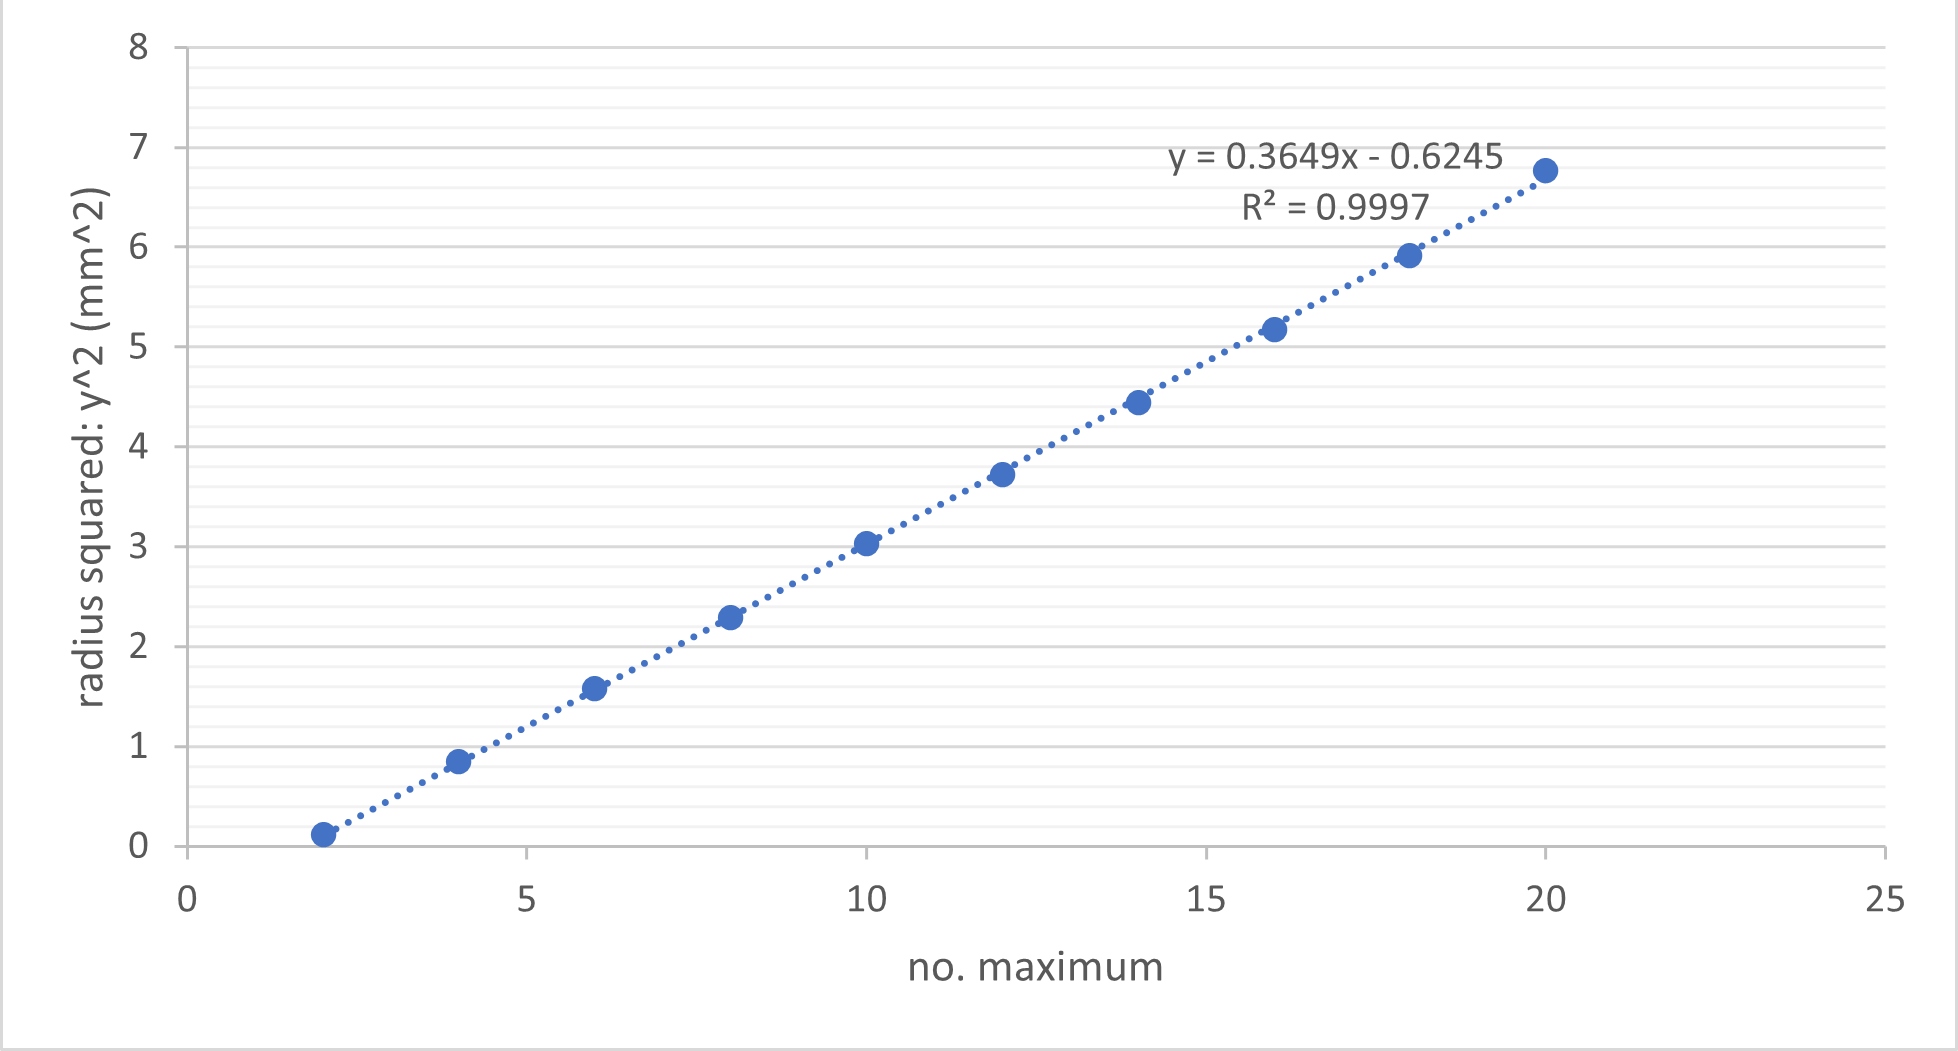
\includegraphics[width=16cm]{./images/imagej_graph.png}
  \caption{$m$ vs. $r^2$ and slope fit obtained through ImageJ analysis}
  \label{fig:result_imagej}
\end{figure}

Note that the $R^2$ value is even lower with this method. Again plugging in the numbers leads to a radius of curvature of the lens of $61.9cm$. 
The difference between the methods is just $6 mm$, thus the both of the measurements seem to agree.

\subsection{Refractive index of water}

To obtain the $\frac{r^2}{m}$ values for water ImageJ was used again, as it was faster. The obtained
values looked like this:

\begin{table}[H]
  \begin{tabular}{lllll}
  Ring Number & Left Hand Side (mm) & Right Hand Side (mm) & Diameter 2y (mm) & $y^2$ ($mm^2$) \\
  \hline
  2           & 2.9710              & 3.7781               & 0.8071           & 0.162852603                                  \\
  4           & 2.524               & 4.224                & 1.7000           & 0.7225                                       \\
  6           & 2.267               & 4.5                  & 2.2330           & 1.24657225                                   \\
  8           & 2.026               & 4.723                & 2.6970           & 1.81845225                                   \\
  10          & 1.838               & 4.994                & 3.1560           & 2.490084                                     \\
  12          & 1.683               & 5.066                & 3.3830           & 2.86117225                                   \\
  14          & 1.511               & 5.22                 & 3.7090           & 3.43917025                                   \\
  16          & 1.374               & 5.375                & 4.0010           & 4.00200025                                   \\
  18          & 1.254               & 5.495                & 4.2410           & 4.49652025                                   \\
  20          & 1.133               & 5.616                & 4.4830           & 5.02432225                                   \\
  \end{tabular}
\end{table}

using regression analysis a value of $\frac{m}{r^2}$ of 3,696721 was obtained. The $R^2$ value was 0.999 which was again very high.\\
\\
Using equation \ref{eq:refractive_index} and the previously obtained curvature of the lens $R = 61.9cm$ (ImageJ result) the refractive index
of the water can be calculated.\\
The resulting value was of 1.349.

\section{Conclusions}

Newton rings could successfully be produced with the setup. Both of the applied measurement techniques were
accurate. They lead to results with a high $R^2$ values. As neither of the two methods is clearly better it comes
down to preference and ease of access/use. \\
\\
The obtained refractive index for water of 1.349 seems plausible when compared to online sources, which provide a 
value of 1.33\autocite{rii}. However the obtained value seems to be quite a bit off the value given online. This could
be due to the water used having a slightly different refractive index than pure water (maybe due to impurities, etc.).\\
As the difference is quite big it is also likely that there where some systematic errors within in the expirement.\\
One problem could be the that the camera was slightly moved between photographing the ruler and the fringe pattern, which
would through all measurements off by the same amount. A different option could be that the the light is not perfectly
parallel, which would distort the image. Similarly distortions could be caused by the different parts of the expiriment not
being aligned properly with each other.\\
If this method was used to determine the refractive index of a material it would help if the radius of the lens was known
beforehand through other means. It prevent errors from the the subsequent experiments to stack up. Furthermore it would also
allow the verification of the setup by examining the calculated refractive index vs. a known one (e.g. air).

\section{Declaration}
I certify that this report has been written by myself, except where otherwise
indicated

\printbibliography


\end{document}
